\section{JSLint}

%-----------------------    ---------------------------------

\begin{frame}
\frametitle{¿Qué es JSLint?}

\begin{itemize}
   \item \texttt{lint} es una herramienta de ayuda al programador
   \item \texttt{lint} se utiliza para detectar código sospechoso, confuso o incompatible entre distintas arquitecturas en programas escritos en C (no detectado por el compilador)
   \item Se basa en análisis estático de código fuente
   \item JSLint permite analizar código JavaScript (y estructuras JSON)
   \item Es una herramienta on-line (aunque se puede descargar y ejecutar en local)
\end{itemize}

\end{frame}


%-----------------------    ---------------------------------

\begin{frame}
\frametitle{JSLint}

\begin{center}
  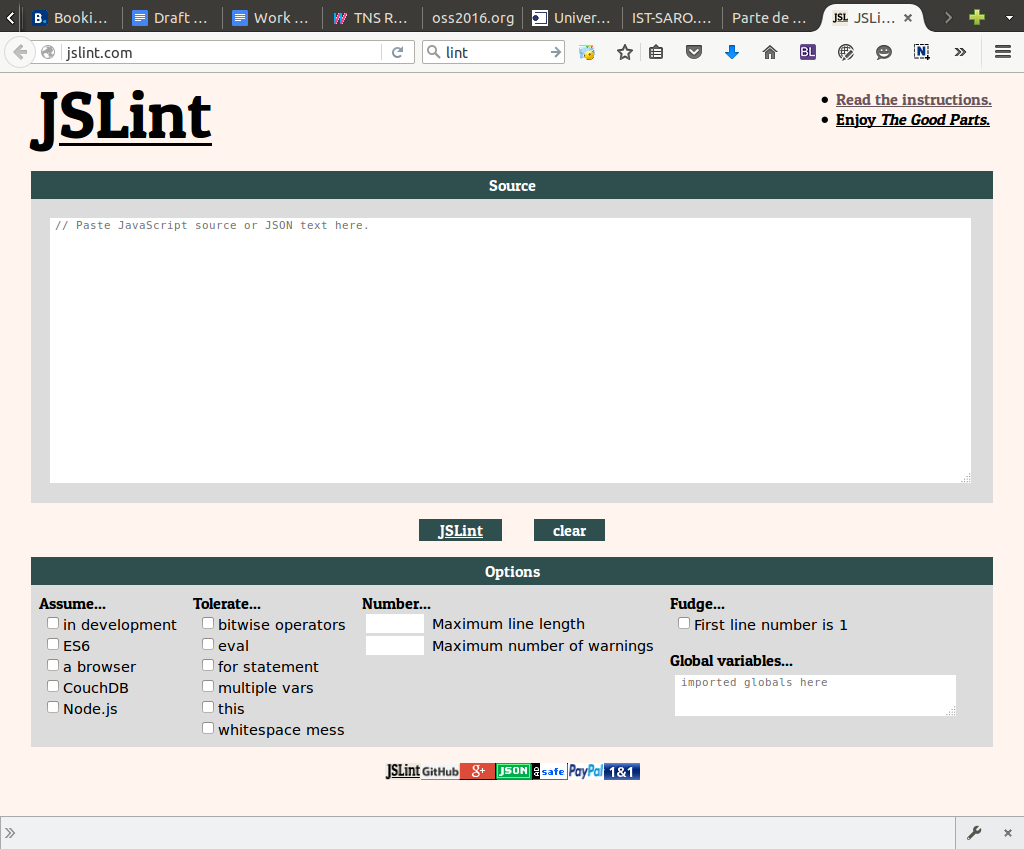
\includegraphics[width=10cm]{figs/jslint.png}
\end{center}


\begin{flushright}
{\tiny
Source: http://jslint.com/
}
\end{flushright}

\end{frame}

